\chapter{Fabrication and Self-Assembly of Exotic Colloids}
\label{ch:exotic}

\section{Introduction}

Stop-flow lithography (SFL) has been demonstrated to be useful for fabricating particles with 
simple geometric and chemical anisotropies, such as a high aspect ratio and 
two-sided Janus functionality.
With this shown, the next question becomes, can the same technique be used to produce other forms of 
anisotropy?  In this chapter, the fabrication of particles with branched anisotropy is explored, and 
the hydrophobic self-assembly of these particles is demonstrated in polar solvent.  More exotic 
functionalities are also explored, including particles whose assembly may take different forms 
depending on the driving force.


\section{Experimental Procedure}
\label{sec:SFLx3}

\subsection{Three-Stream Experiment}

\figone{fig:three-stream}{figures/complex-shapes/three-stream-fab.jpg}{0.6\linewidth}{
Fluorescence image of a microchannel during three-stream flow.}

SFL experiments were carried out using the device design described in Section~\ref{sec:sfl-expt-rods} 
(see Figure~\ref{fig:device-design}).  All three input channels were used for the fabrication of 
branched and other exotic particles, with the typical monomer inputs being PEGDA solution in
the center channel and TMPTA solution on the left- and right-hand inputs. (See 
Section~\ref{sec:janus-materials} for a full description of these solutions.) 
Typical initial pressures for microchannel
flow were 8 $psi$ for the left- and right-hand inputs and 6 $psi$ for
the center input. Typical values for $t_{flow}$, $t_{pause}$ and $t_{expose}$ were 2.0 s, 2.0 s and 0.25 s, 
respectively.  SFL fabrication masks were designed for three-stream fabrication in a manner similar to 
the masks used for the fabrication of Janus rods, with several identical particle patterns arranged
in a single line.  These masks could then be aligned to allow polymerization overlapping the 
two parallel TMPTA/PEGDA interfaces.

All SFL parameters were adjusted at the beginning of each experiment to optimize fabrication 
conditions.  A number of constraints were applied in order to achieve consistent results for 
the fabrication of multiple-component particles, including:

\begin{itemize}
\item $t_{flow}$ sufficient to eject particles following polymerization.
\item $t_{pause}$ sufficient for a complete stop in flow, to optimize polymerization conditions.
\item $t_{pause}$ small enough to prevent the center stream from breaking up into droplets.
\item $t_{expose}$ sufficient to fully cure particles.
\item Relative pressures optimized to produce a jetting flow with a sufficiently narrow stream
for fabricating small particles.
\end{itemize}

The major difficulty in this experiment was balancing the relative pressures and flow times to produce
PEGDA/TMPTA interfaces which were sufficiently narrow for the fabrication of the particles of interest
while still avoiding the break-up of the center stream into a series of droplets (``dripping mode'').
This set of constraints imposed strict limits on the minimum size of the particles, with
the minimum width achieved for the center stream being approximately 12 \microns.
Due to the presence of air bubbles and imperfections in the microchannel, this optimization had to be
performed for every experiment and greatly reduced consistency between subsequent fabrication experiments.

\subsection{Collection and Processing}

Complex Janus particles were ejected from the fabrication channel while still in monomer solution and collected
in an open reservoir.  The particle collection procedure was identical to that outlined in 
Section~\ref{sec:exp-collection}. Ethanol was used as the collection solvent, and glass Pasteur
pipettes were used to extract the particles.  All particles samples
were washed by microcentrifuge solvent exchange using ethanol, and were transferred to 
glass observation
chambers in either ethanol (for simple fluorescence observation) or in water (for
observation of self-assembly).


\section{Results and Discussion}

\subsection{Branched Particles}

\figone{fig:branching-anisotropy}{figures/complex-shapes/branching-particles-anisotropy-dimension.png}{0.6\linewidth}{
Anisotropy dimension: branching.~\cite{glotzer-solomon}}

SFL fabrication experiments were performed with masks designed to target the branching morphologies
portrayed in the scheme of anisotropy dimensions outlined by Glotzer and Solomon
(see Figure~\ref{fig:branching-anisotropy}).~\cite{glotzer-solomon}  As single-component rods and 
two-part Janus rods had been accomplished in Chapter~\ref{ch:rods}, the following particle 
morphologies were targeted: hydrophilic rods with hydrophobic patches on either end, three-branch particles
with hydrophobic ends, and four-branch particles with hydrophobic ends.


\begin{figure}[h]
\begin{center}
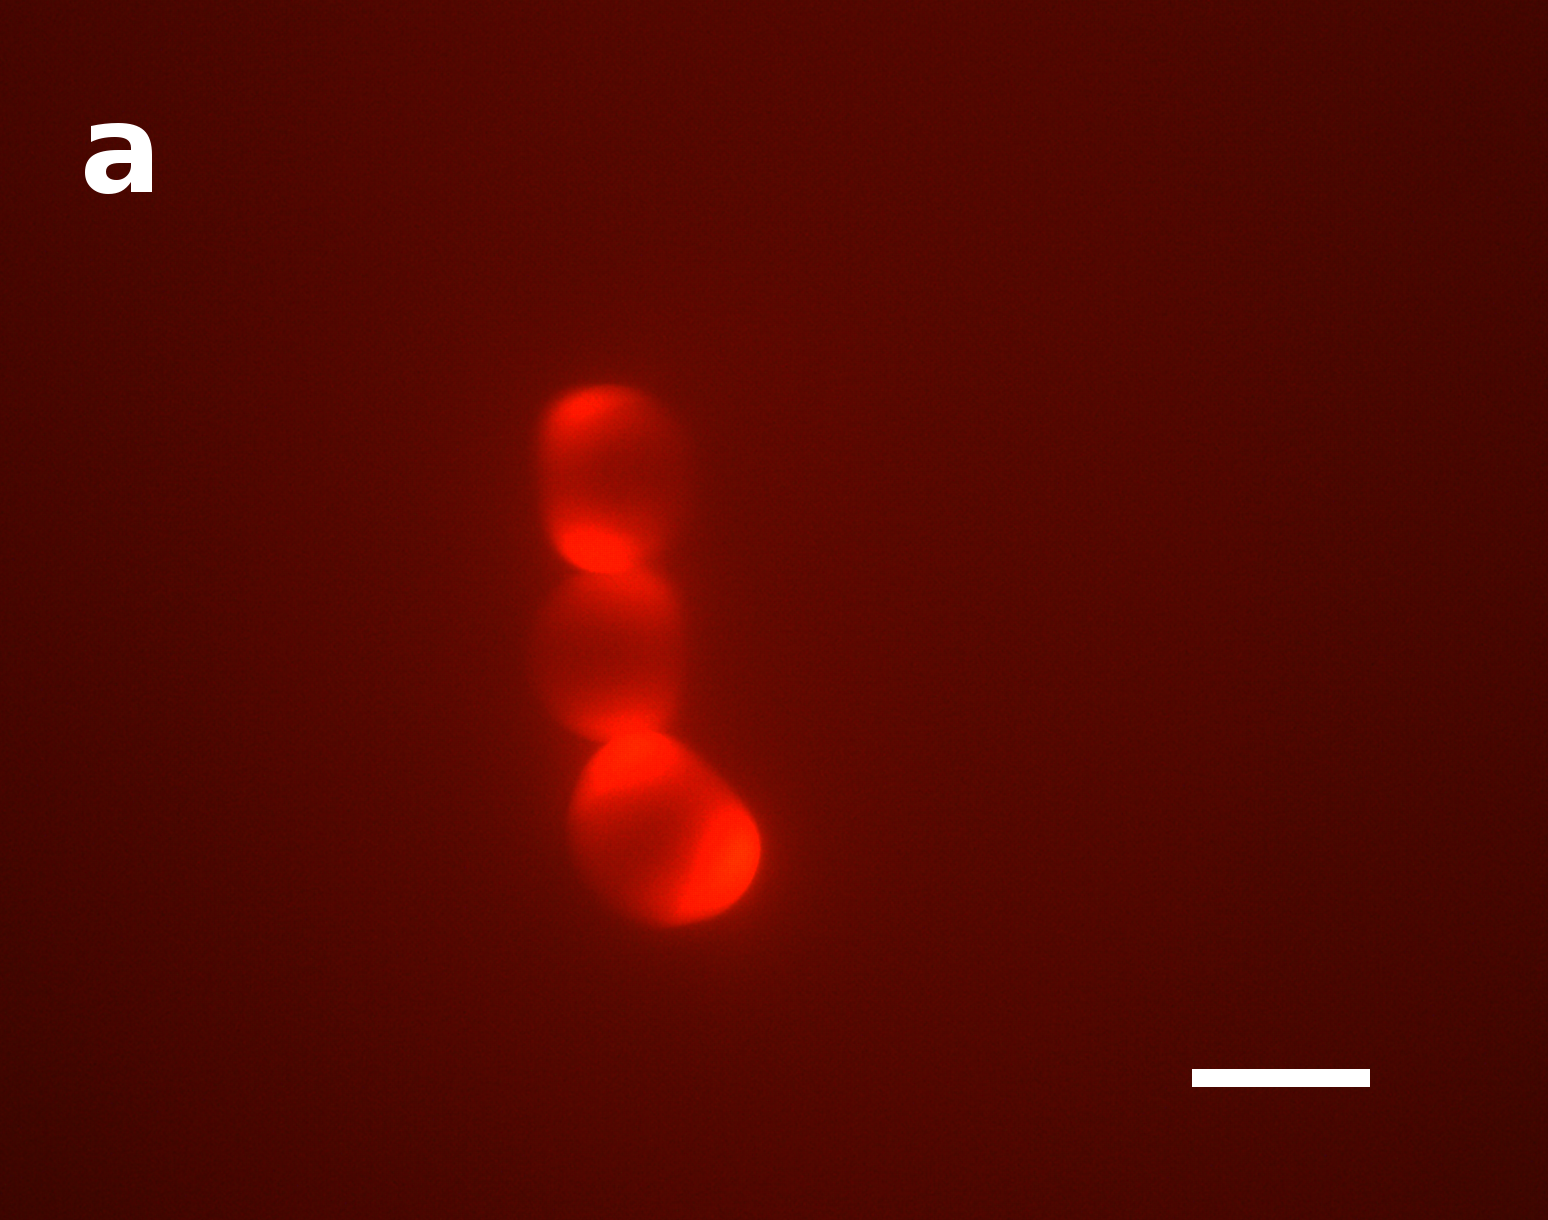
\includegraphics[height=1.5in]{figures/complex-shapes/twopatch-3chain-sb20.png} 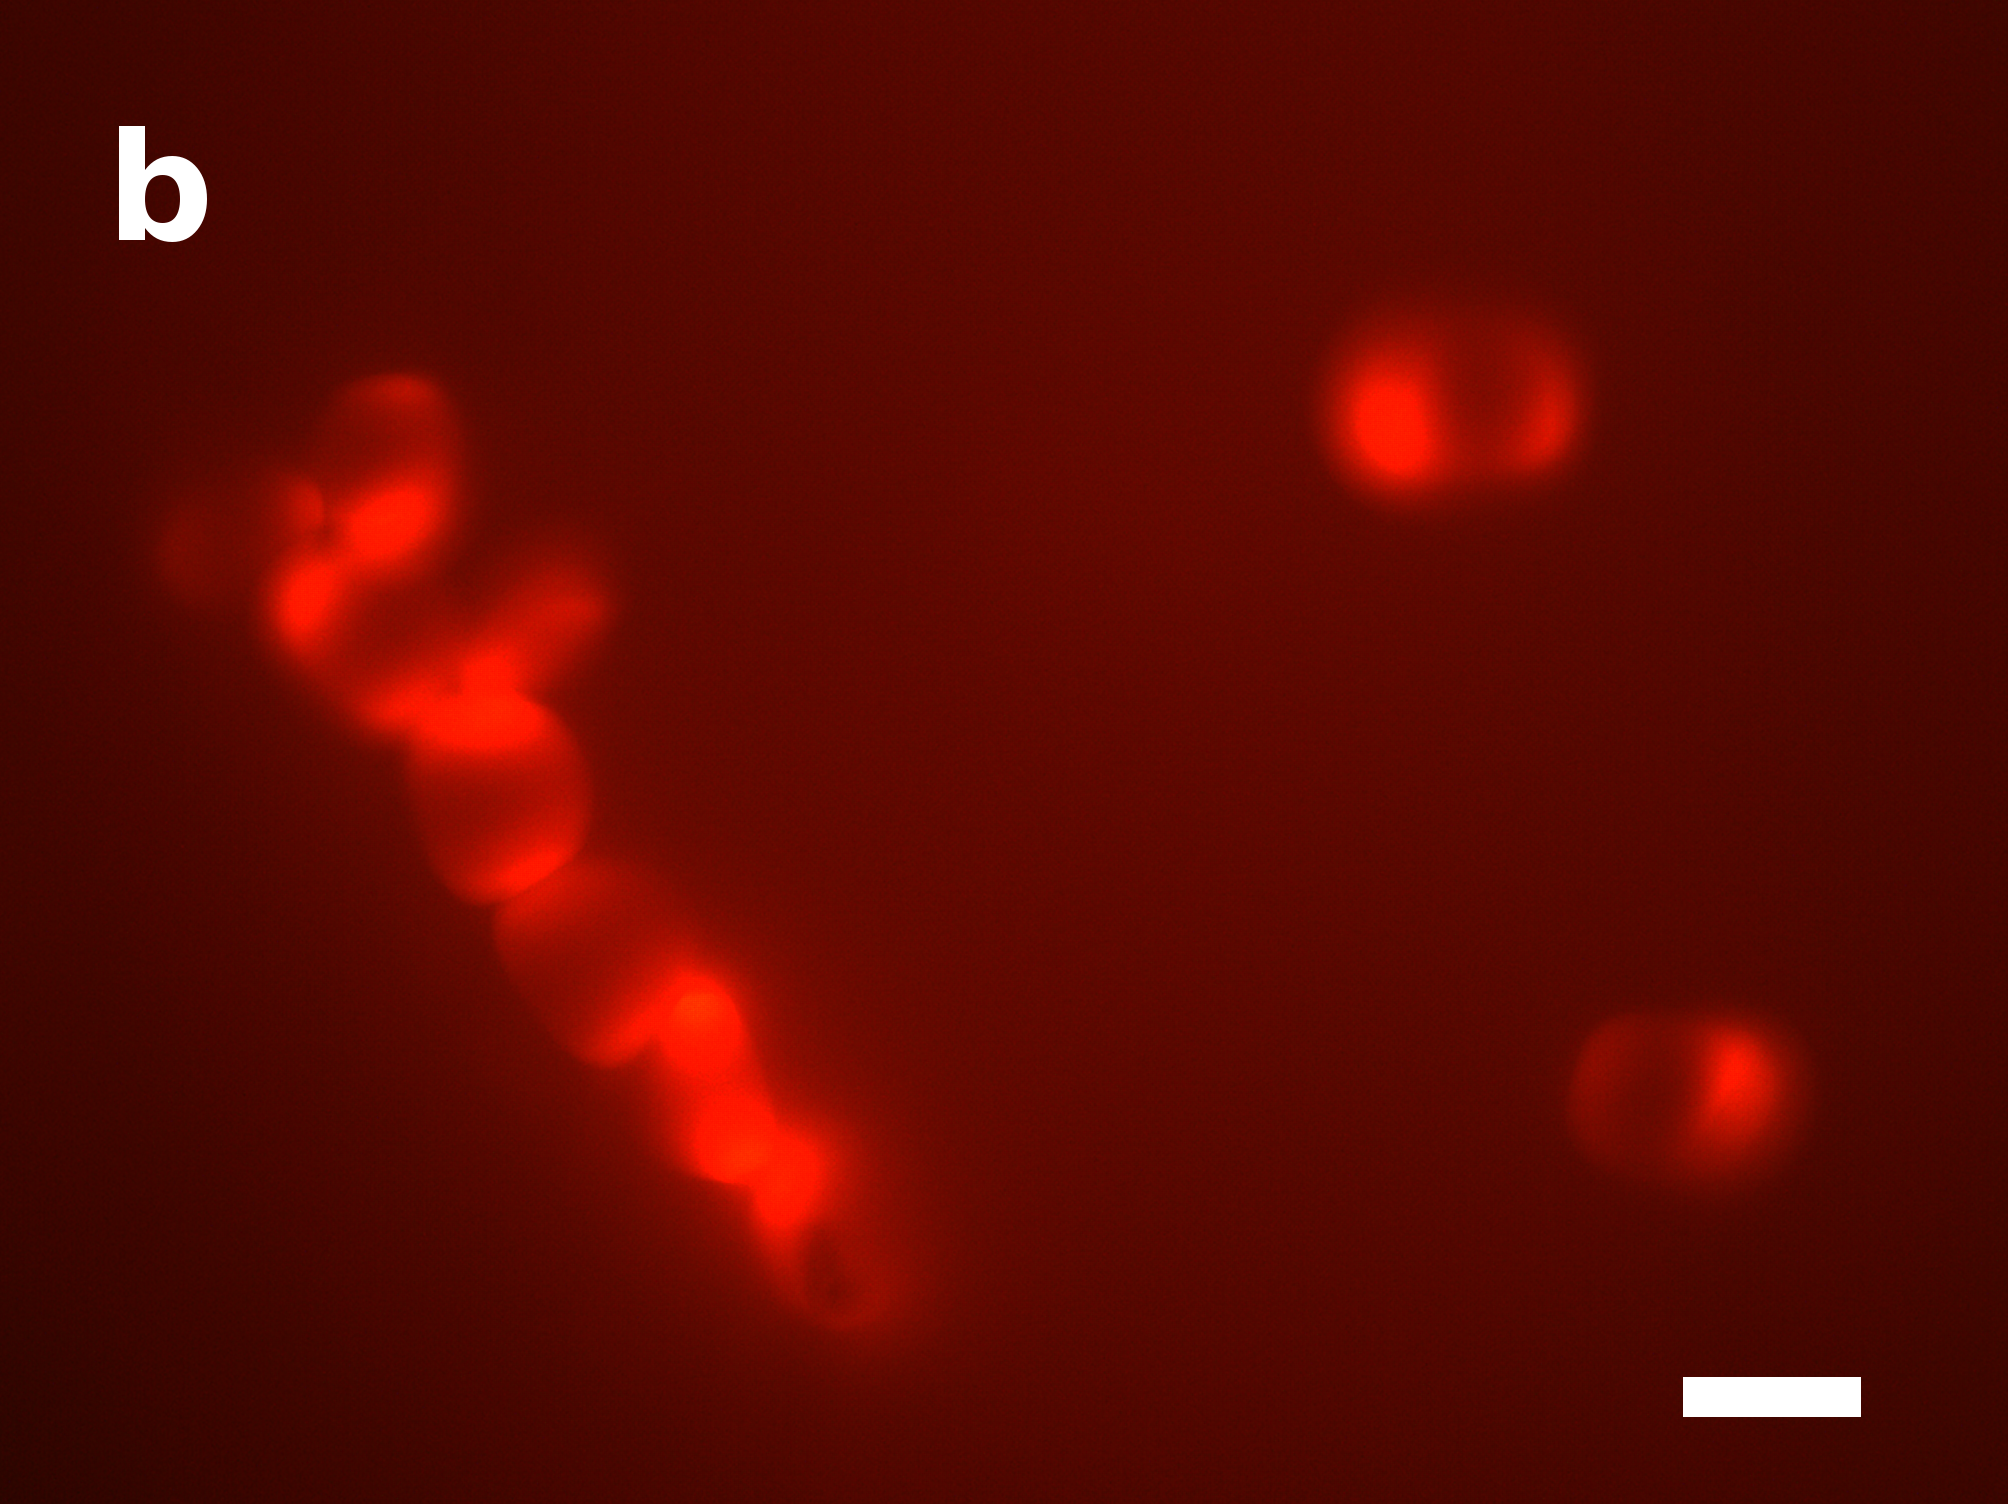
\includegraphics[height=1.5in]{figures/complex-shapes/twopatch-flchain-sb20.png}
\end{center}
\caption{Chain-like assembly of tall two-patch particles. Scale-bar is 20 \microns.}
\label{fig:tall-2patch}
\end{figure}

\begin{figure}[h]
\begin{center}
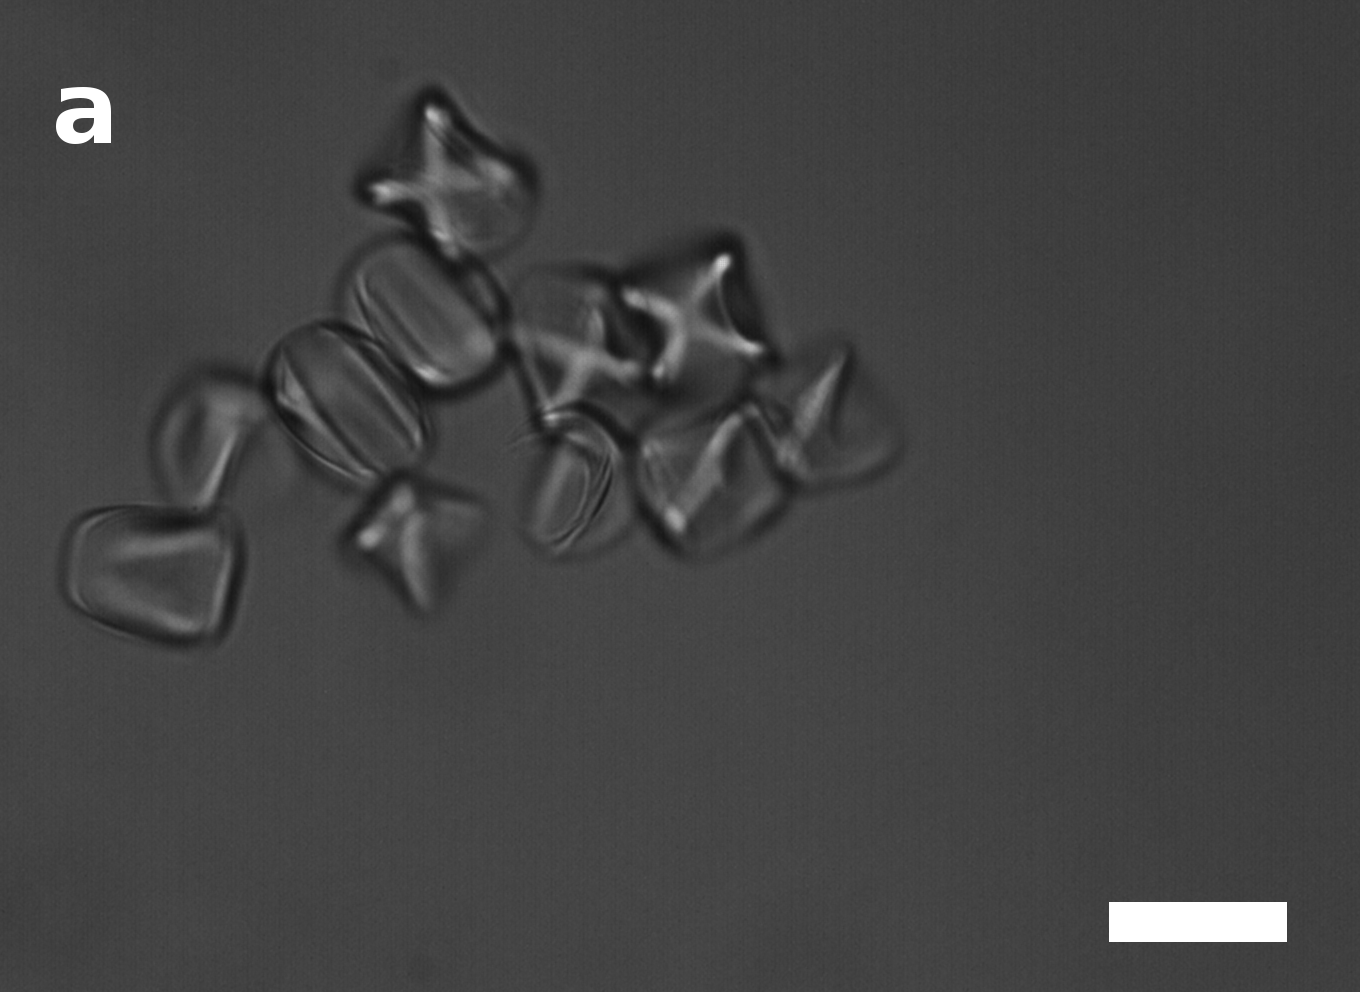
\includegraphics[height=1.5in]{figures/complex-shapes/4patch-sb20-01.png} 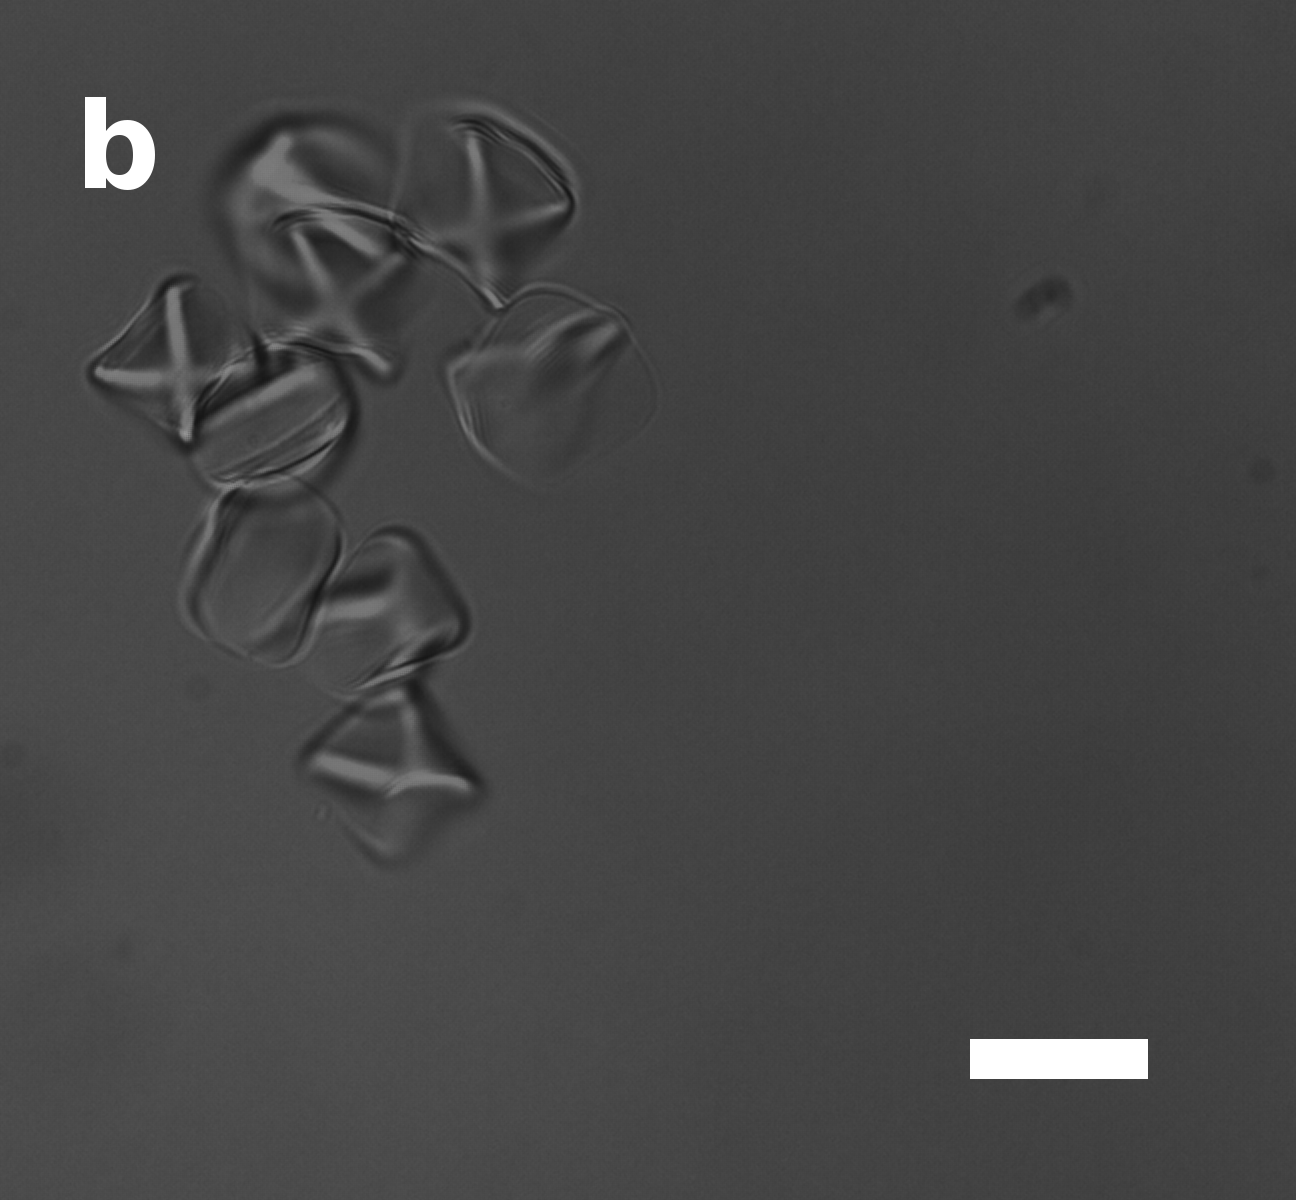
\includegraphics[height=1.5in]{figures/complex-shapes/4patch-sb20-02.png} 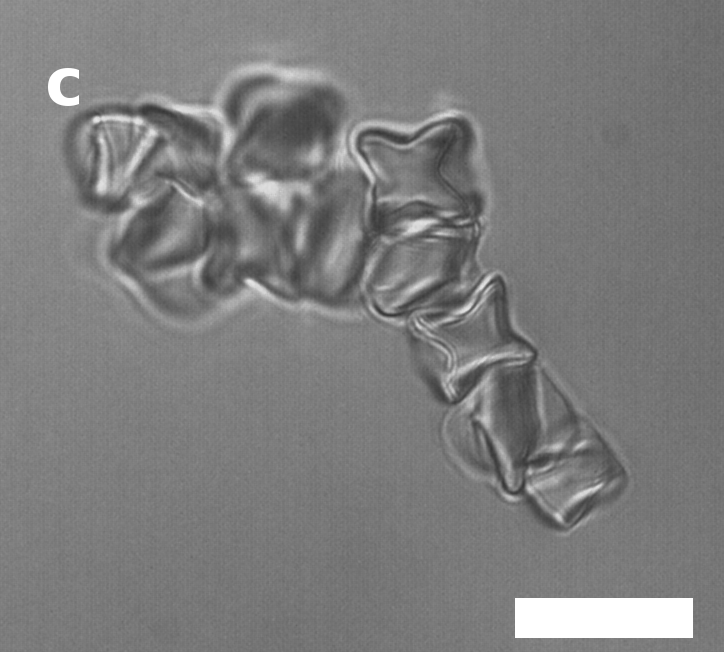
\includegraphics[height=1.5in]{figures/complex-shapes/4patch-sb20-03.png}
\end{center}
\caption{Self-assembly of tall four-patch particles. Scale-bar is 20 \microns.}
\label{fig:tall-4patch}
\end{figure}

As with Janus rods, initial experiments were carried out in ``tall'' microchannel devices with a height of
15 \microns~to produce larger particles which might be more easily studied.  These proof-of concept
experiments were carried out to produce two-patch and four-patch particles with heights of roughly 11
\microns~and width of 20 \microns.  

These particles were then transferred into water suspension to 
study self-assembly.  Two-patch particles were observed to form linear chain-like structures
with end-to-end assembly, as seen in Figure~\ref{fig:tall-2patch}.  This is dramatically different from
the micelle-like clusters formed by Janus rods, shown previously in 
Figure~\ref{fig:assembly-small-clusters}.  Four-patch particles assembled into denser clusters due
to their additional assembly sites, producing structures which combined chain-like 
morphologies (Figure~\ref{fig:tall-4patch}(c)) with dense and loop-like structures 
(Figure~\ref{fig:tall-4patch}(a,b)).

\begin{figure}[h]
\begin{center}
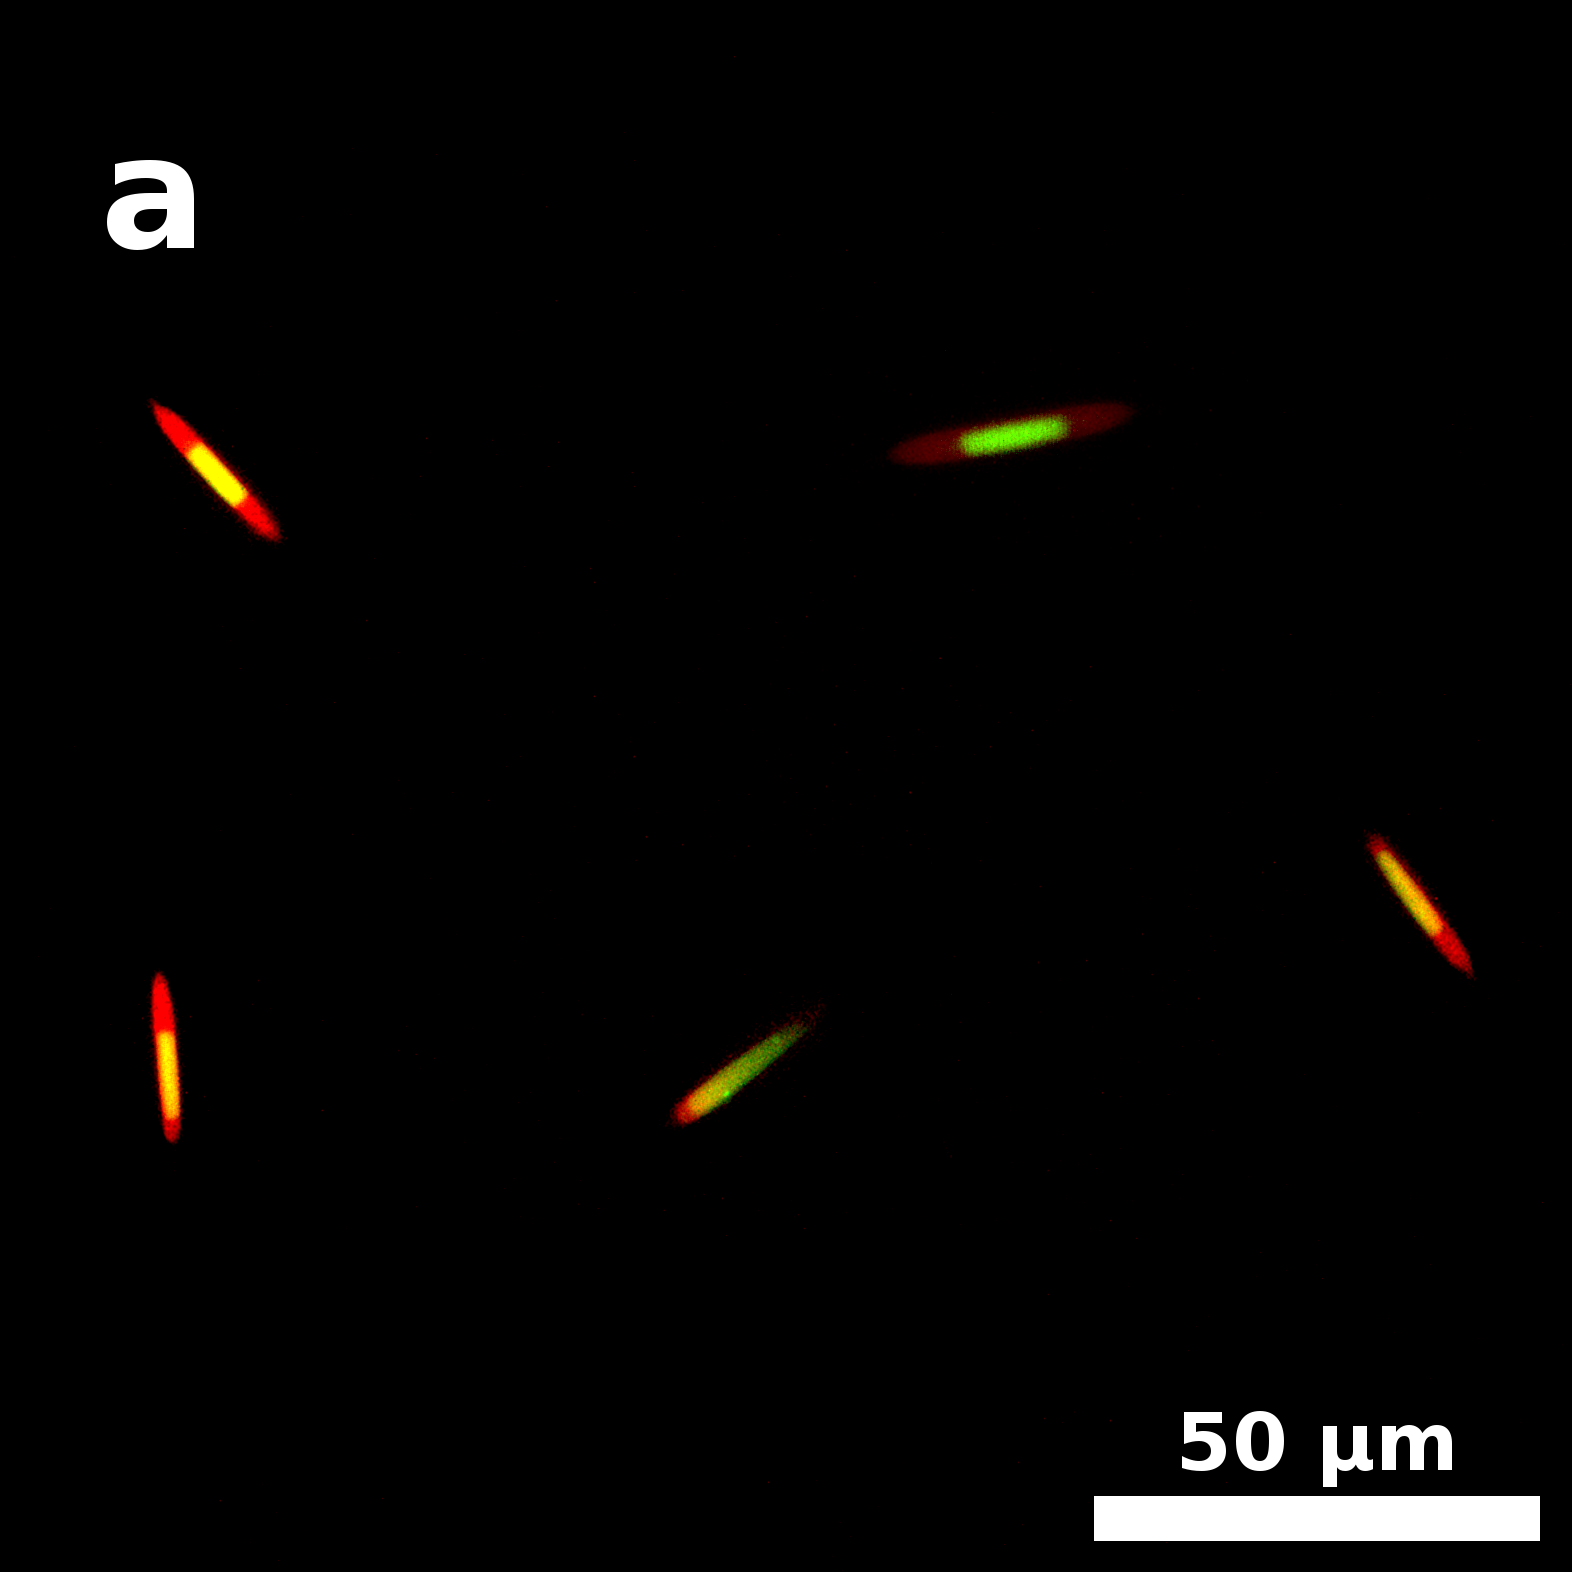
\includegraphics[height=1.5in]{figures/complex-shapes/two-patch-rods-single-image.png} 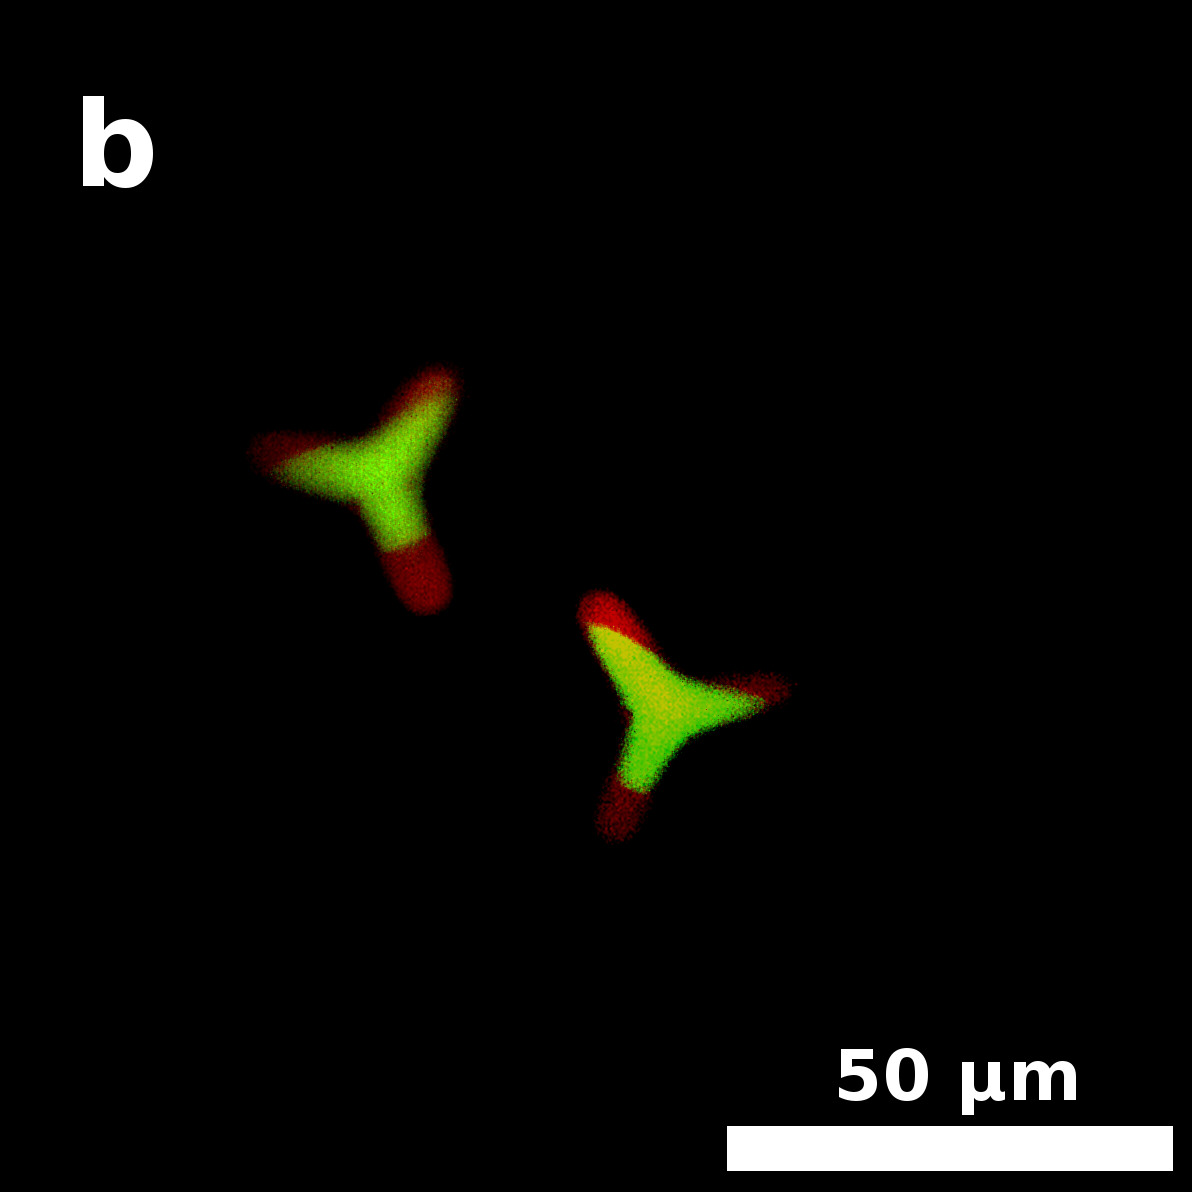
\includegraphics[height=1.5in]{figures/complex-shapes/janus-threepatch-single-image.png} 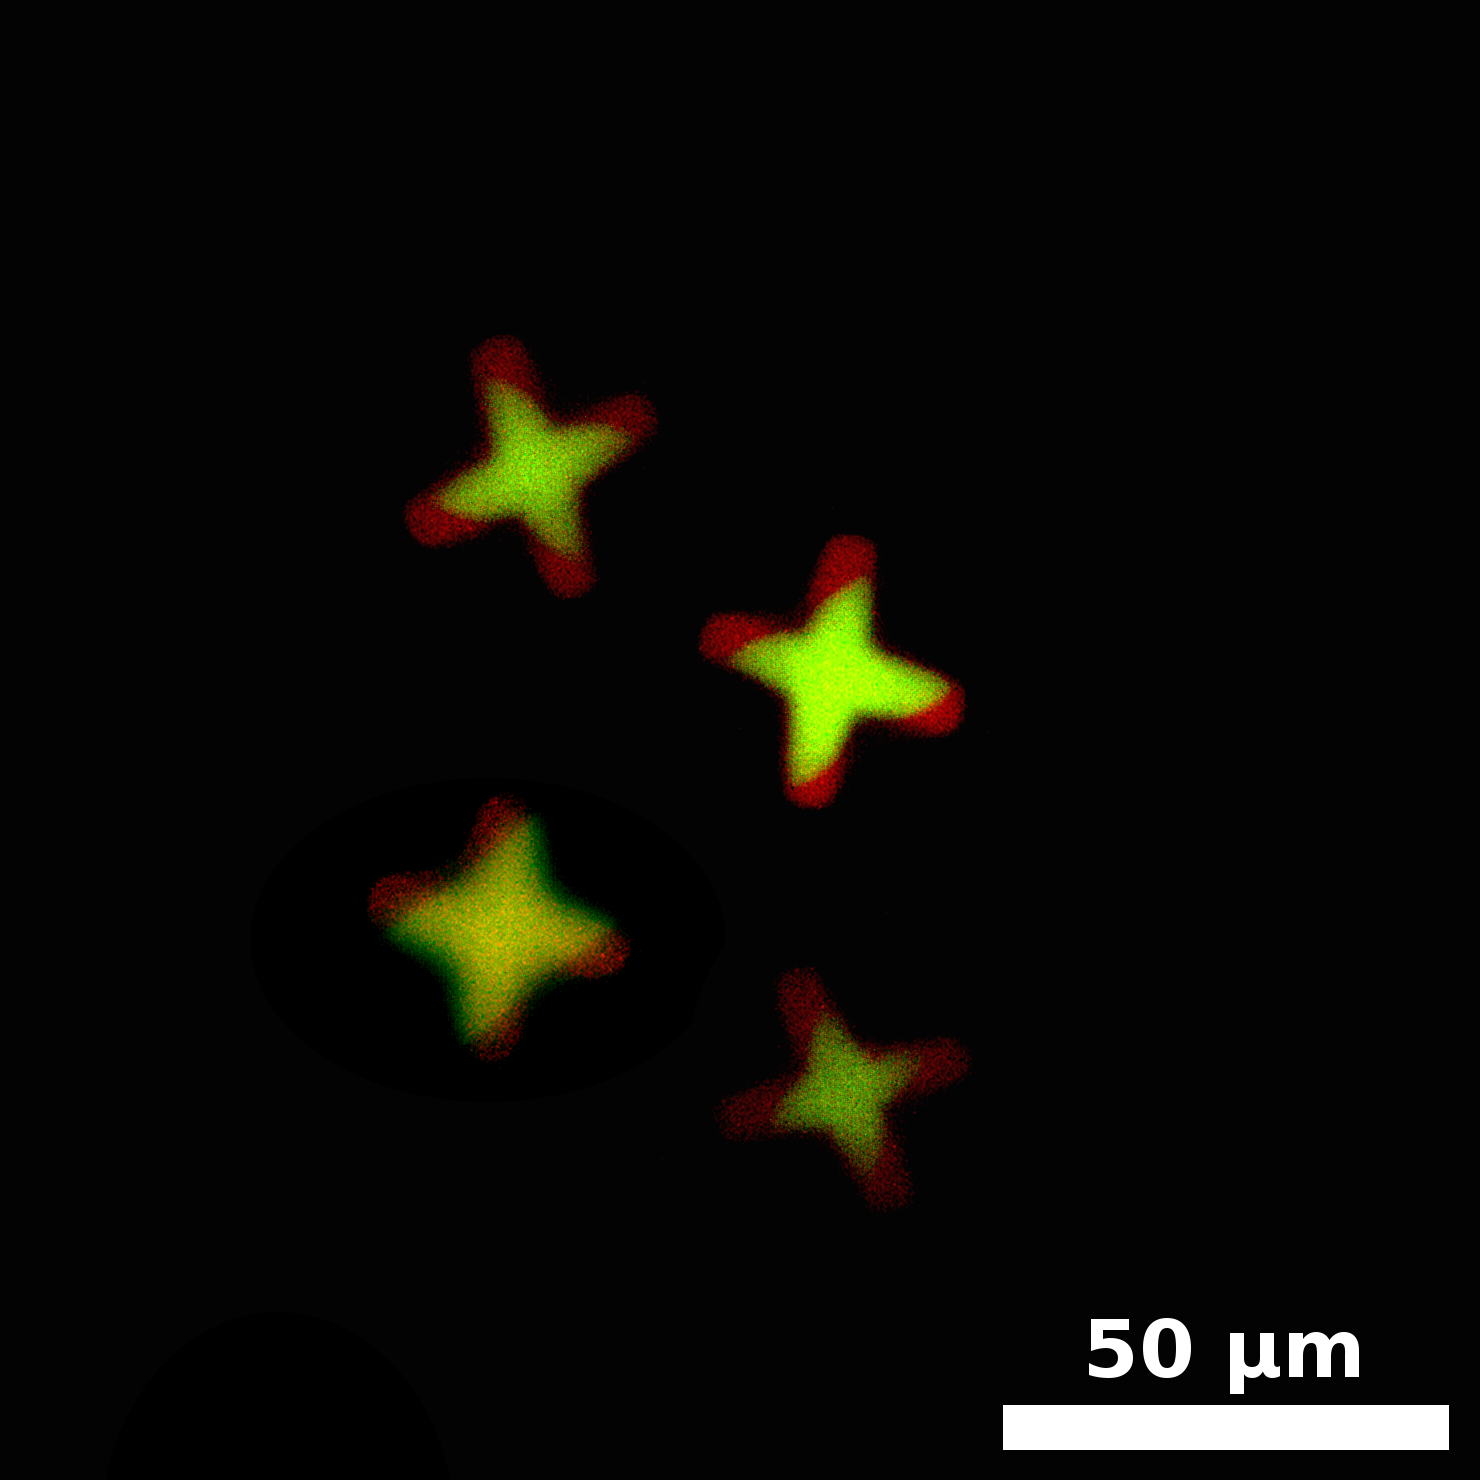
\includegraphics[height=1.5in]{figures/complex-shapes/janus-crosses-single-image.png}
\end{center}
\caption{Two-component particles with (a) two, (b) three and (c) four hydrophobic patches.}
\label{fig:branched-series}
\end{figure}

\begin{figure}[h]
\begin{center}
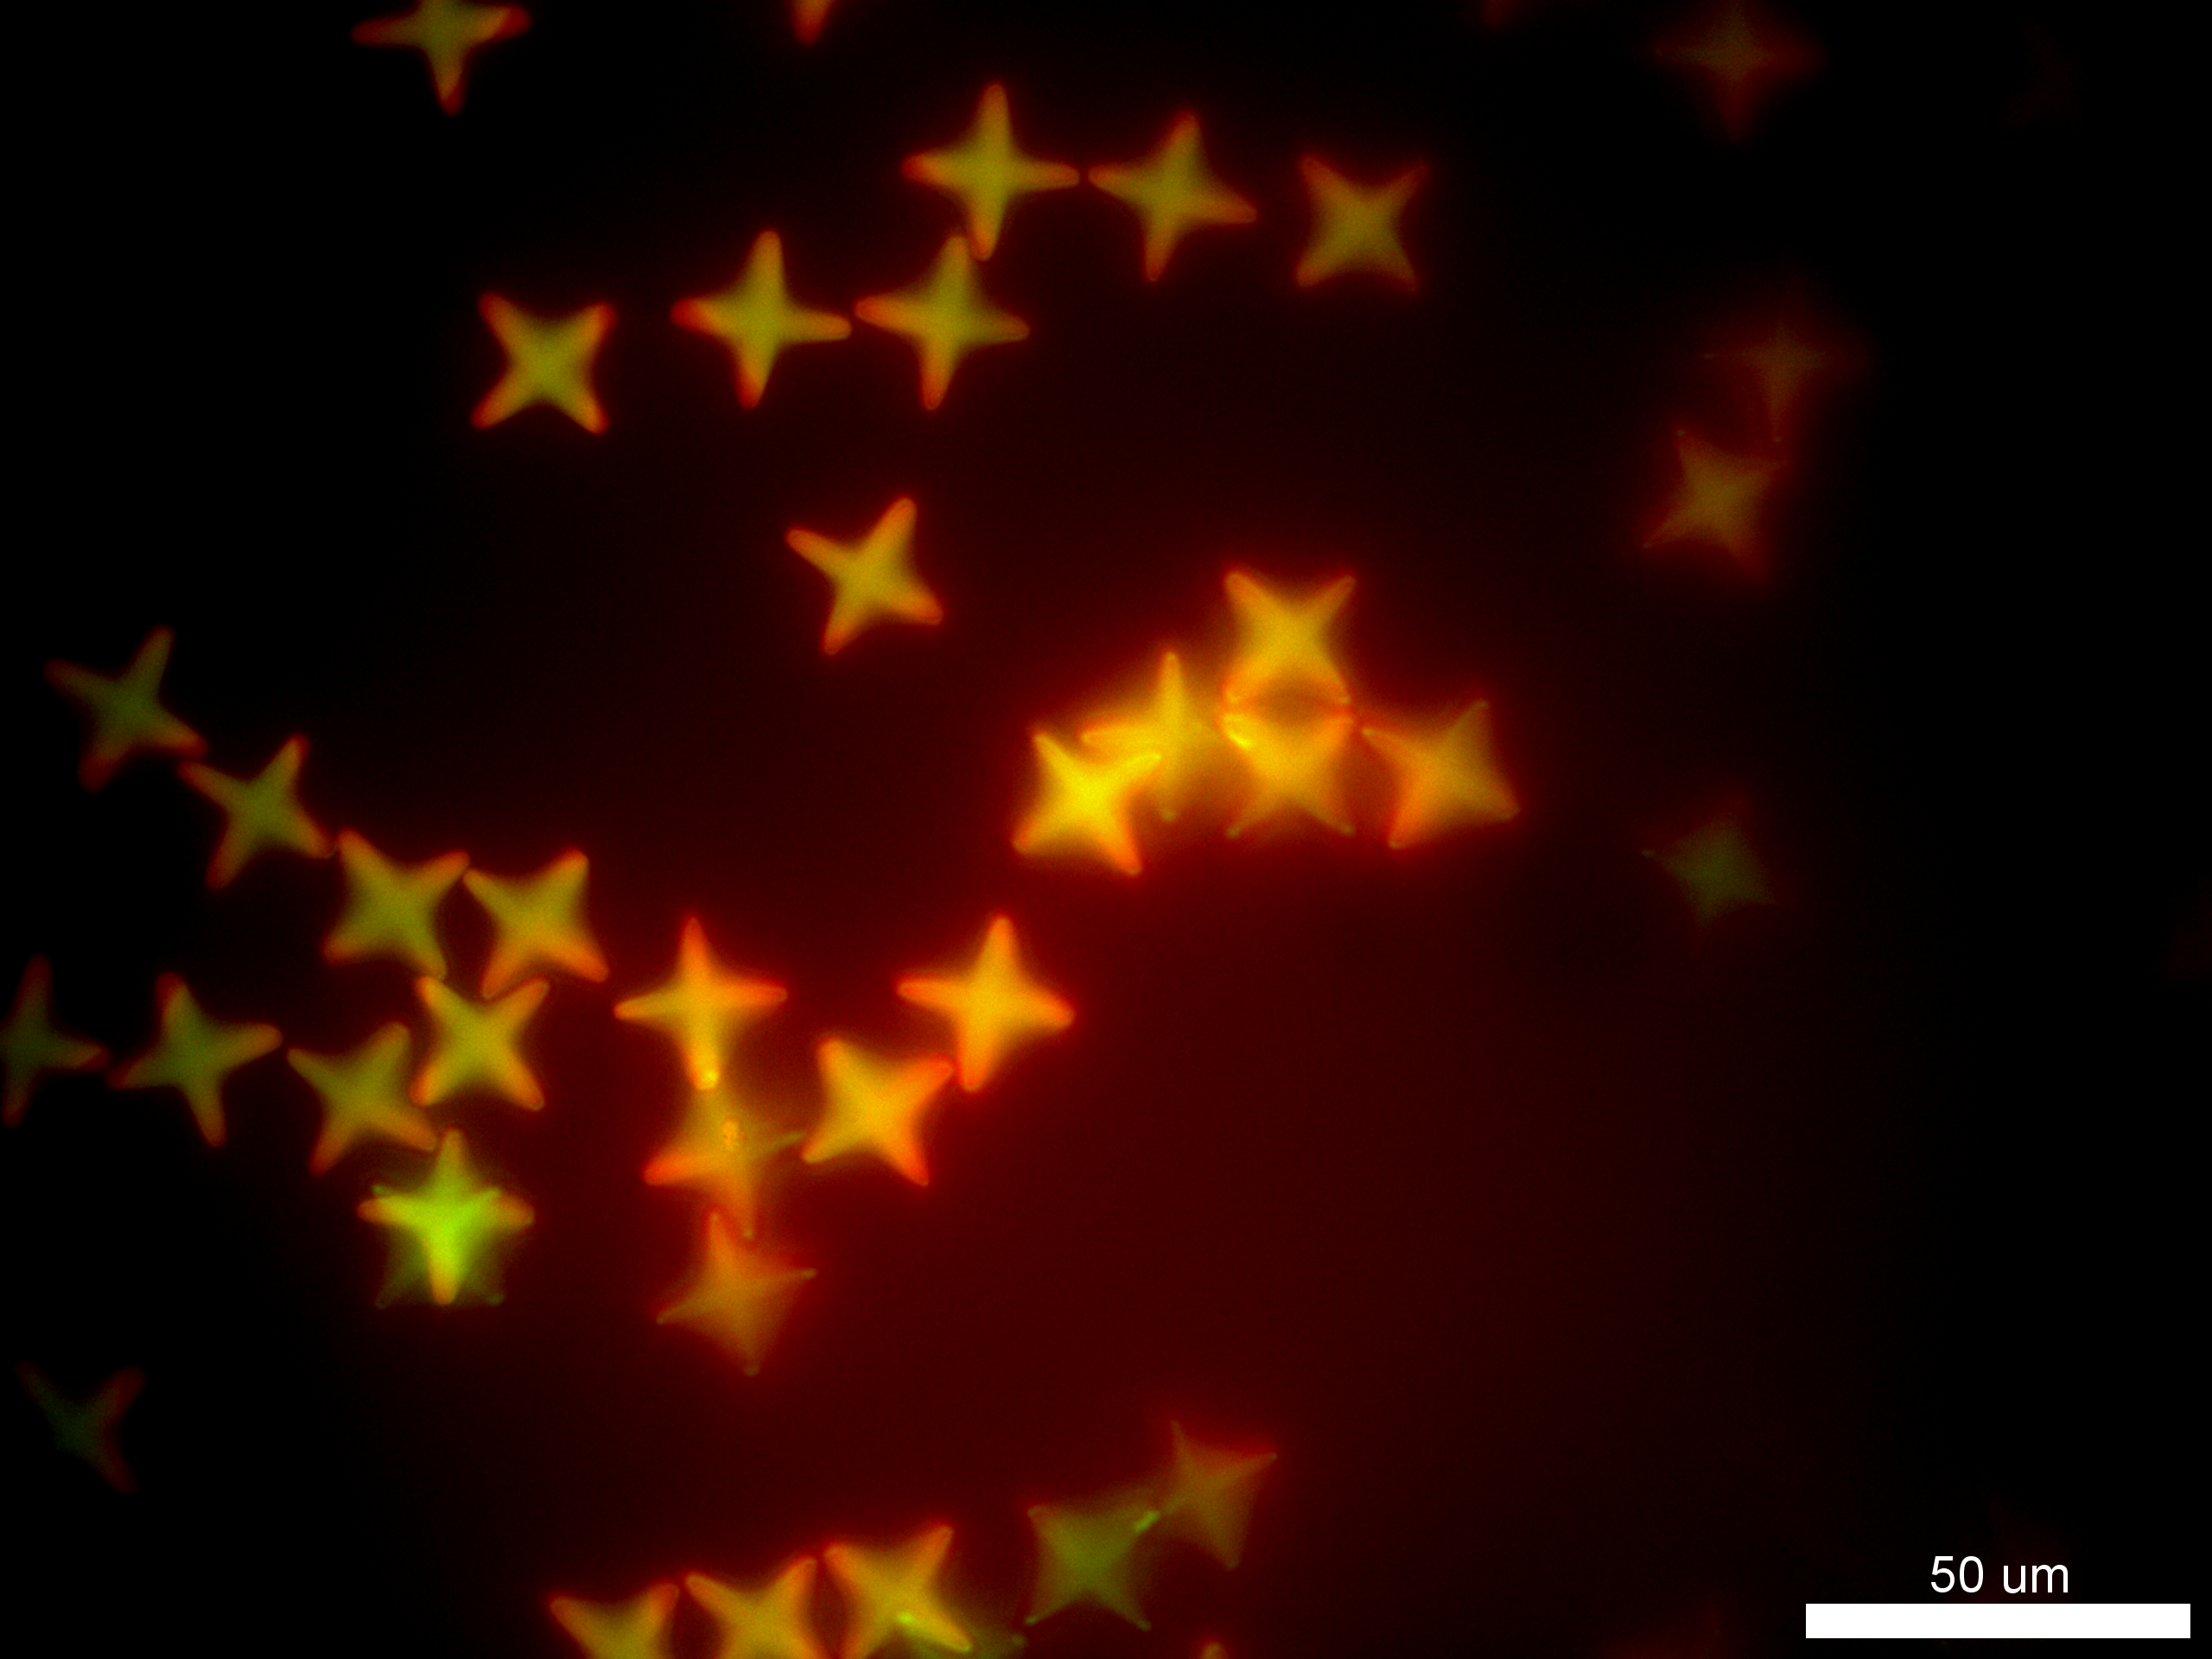
\includegraphics[width=0.6\linewidth]{figures/complex-shapes/crosses-high-conc.png}
\end{center}
\caption{Janus crosses are suspended at high concentration and self-assemble by contact
of hydrophobic ``patches'' at the end of each arm..}
\label{fig:crosses-high-conc}
\end{figure}

Following this demonstration, subsequent experiments focused on producing high-quality 
branched Janus particles using microchannels with a height of 7 \microns.  These experiments were carried
out to produce representative 
examples of particles with two, three and four patches with heights of
3 \microns~and lateral dimensions of approximately 30 \microns.  

Unfortunately, due to the considerations
outlined in Section~\ref{sec:SFLx3}, these experiments failed quickly and rarely produced more than a few
particles at a time.  One relatively large sample of a 3000 four-patch ``crosses'' was successfully fabricated 
and suspended in water to observe their self-assembly; a fluorescence 
microscopy image of this sample is shown in Figure~\ref{fig:crosses-high-conc}.  Here we can see 
some strongly-aligned self-assembly, with crosses generally arranging themselves such that
their hydrophobic ends are maximizing contact area.  This is a flexible mode of self-assembly, 
which may enable the formation of many different superstructures, and this image alone shows several different
cluster morphologies.

\subsection{Multiple Modes of Assembly}

\begin{figure}[h]
\begin{center}
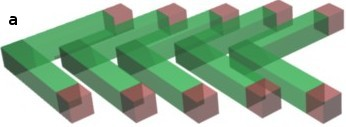
\includegraphics[width=0.4\linewidth]{figures/complex-shapes/boomerangs-dense-assembly.jpg} \hfill 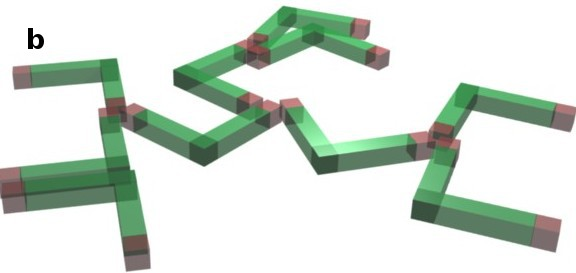
\includegraphics[width=0.4\linewidth]{figures/complex-shapes/boomerangs-open-assembly.jpg}
\end{center}
\caption{Two possible modes of self-assembly for Janus ``boomerangs'': (a) geometric, and (b) open and hydrophobic}
\label{fig:boomerang-assembly}
\end{figure}

In addition to the branched particles illustrated above, we attempted to design and fabricate 
a particle which might undergo two or more different types of self-assembly depending on the environment
in which it was placed.  

To achieve this, we designed a ``boomerang'' particle incorporating 
hydrophobic ends.  Under neutral solvent conditions, such as a weakly-polar solvent such as DMSO, these particles
might be induced to undergo a 
dense geometric self-assembly with cluster morphology dictated by the 
particle shape. An example of such a structure is illustrated in Figure~\ref{fig:boomerang-assembly}(a).
Such an assembly might be induced by the introduction of a low-molecular-weight polymer to induce a 
depletion interaction.  To achieve the second assembly mode, the particles would be 
placed in a strongly-polar solvent such as water in order to drive a hydrophobic attraction between 
the particle ends, thus producing a more randomly-oriented and open structure such as the one illustrated
in Figure~\ref{fig:boomerang-assembly}(b).

\figone{fig:boomerangs}{figures/complex-shapes/janus-boomerangs-single-image.jpg}{0.7\linewidth}{
Fluorescence image of Janus ``boomerangs'' suspended in DMSO.}

Large boomerang-type particles were successfully fabricated by SFL and imaged via fluorescence 
microscopy (see Figure~\ref{fig:boomerangs}).  However, while these particles were successfully 
observed in DMSO, we failed to observe an depletion-driven geometric
self-assembly. We attempted to transfer a sample of boomerang particles to water to observe
hydrophobic assembly, but failed due to particle transfer issues (see Section~\ref{sec:rod-collection}).
